\documentclass[a4paper]{article}
\usepackage[top=1in, bottom=1.25in, left=1.25in, right=1.25in]{geometry}
\usepackage{amsmath}
\usepackage{multicol}
\usepackage{graphicx}
\RequirePackage{ltxcmds}[2010/12/07]
\graphicspath{{./images/}}
\usepackage{float}
\usepackage{amsfonts}
\title{BPSK system}
\author{ }

\begin{document}

\maketitle


This document describes the simulation of a Key Distribution in back-to-back configuration. The signal is generated by the system described in the \textit{MQAM\_system.pdf} document, as such the blocks described in that document will not be described here. 

\section{System to analyse}

In this step on our work we are attempting to simulate a \textit{back-to-back} QKD setup, in which the signal output by the emitter is directly fed into the receiver.
\par
For simplicity, in this early stage we have chosen to use a BPSK coding. This is a simplified setup but still allows us to study the effect of the relative phase between the local oscillator and the signal.
\par
A simplified diagram of the system being simulated is presented in the Figure~\ref{fig:physicalsystem}. In broad terms, our QKD simulation is required to be able to send a random bit sequence (the key) by means of an optical signal, accomplish a full key reconstruction from the optical signal and subsequently perform a key security check through the evaluation of the Bit Error Rate (BER).

\begin{figure}[h]
\centering
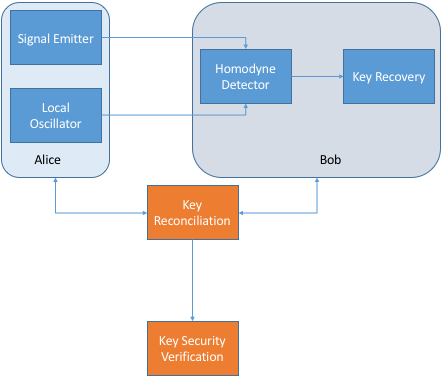
\includegraphics[width=.6\linewidth]{PhysicalSystem.png}
\caption{Overview of the QKD system being simulated.}
\label{fig:physicalsystem}
\end{figure}

In the next section we will show that our simulation can currently accomplish all of the proposed objectives.

\section{Numerical model}

The current simulation can be visually interpreted by the block diagram presented in Figure~\ref{fig:simulatedsystem}. In this section we will go into some detail on the workings of the blocks responsible for the Signal detection and Key reconstruction (i.e. all blocks other than \textbf{MQAM Transmitter} and \textbf{Local Oscillator}).

\begin{figure}[h]
\centering
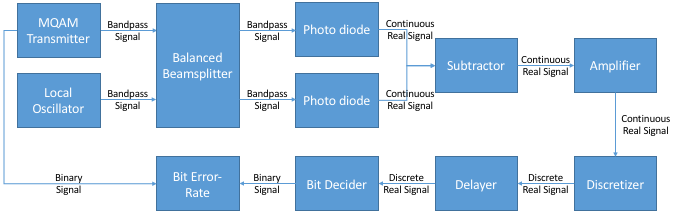
\includegraphics[width=\linewidth]{simulatedsystem.png}
\caption{Visual representation of the simulated system.}
\label{fig:simulatedsystem}
\end{figure}

Along the description of each block, we include the crucial coding (the code responsible for setting the signal parameters is omitted) and a figure showing the output of each block.

\subsection{Local Oscillator}

\subsubsection*{Input Parameters}

\begin{multicols}{2}
	\begin{itemize}
		\item LocalOscillatorPhase
		\item LocalOscillatorOpticalPower
		\item \verb|LocalOscillatorOpticalPower_dBm|
	\end{itemize}
\end{multicols}

\subsubsection*{Functional Description}

This blocks accepts a complex signal (either with XY polarization or a simple Band Pass signal) and outputs a phase constant complex signal with the same length as the input signal. The phase and optical power are defined by the values of \textit{LocalOscillatorPhase} and \textit{LocalOscillatorOpticalPower} respectively.

\subsubsection*{Input Signals}

\textbf{Number}: 1

\textbf{Type}: Complex signal (ContinuousTimeContiousAmplitude)

\subsubsection*{Output Signals}

\textbf{Number}: 2

\textbf{Type}: Complex signal (ContinuousTimeContiousAmplitude)


\subsection{Balanced Beamsplitter}

\subsubsection*{Input Parameters}

\begin{multicols}{2}
	\begin{itemize}
		\item setTransferMatrix
	\end{itemize}
\end{multicols}

\subsubsection*{Functional Description}

This block accepts two complex signals and outputs two complex signals built from a mixture of the two inputs according to a pre-determined and user defined transfer matrix.

\subsubsection*{Input Signals}

\textbf{Number}: 2

\textbf{Type}: Complex signal (ContinuousTimeContiousAmplitude)

\subsubsection*{Output Signals}

\textbf{Number}: 2

\textbf{Type}: Complex signal (ContinuousTimeContiousAmplitude)


% This block takes two input signals, splits them in accordance with the beamsplitter matrix presented in~\eqref{eq:matrix}, and outputs two signals, effectively mixing the two inputs.
%
%\begin{equation}\label{eq:matrix}
%\frac{1}{\sqrt{2}}
%\begin{pmatrix}
%1 & 1\\
%1 & -1
%\end{pmatrix}
%\end{equation}
%
%The following code is run for every pair of values in the input signals.
%
%\begin{verbatim}
%		t_complex x1;
%		inputSignals[0]->bufferGet(&x1);
%		t_complex x2;
%		inputSignals[1]->bufferGet(&x2);
%
%		
%		t_complex x4 = div*(x1 + x2);
%		t_complex x3 = div*(x1 - x2);
%
%		
%		outputSignals[0]->bufferPut(x3);
%		outputSignals[1]->bufferPut(x4);
%\end{verbatim}
%
%The inputs for this block are presented in the Figures~\ref{fig:bsin1}~and~\ref{fig:bsin2} and the outputs in the Figures~\ref{fig:bsout1}~and~\ref{fig:bsout2}.

%\begin{figure}[H]
%\centering
%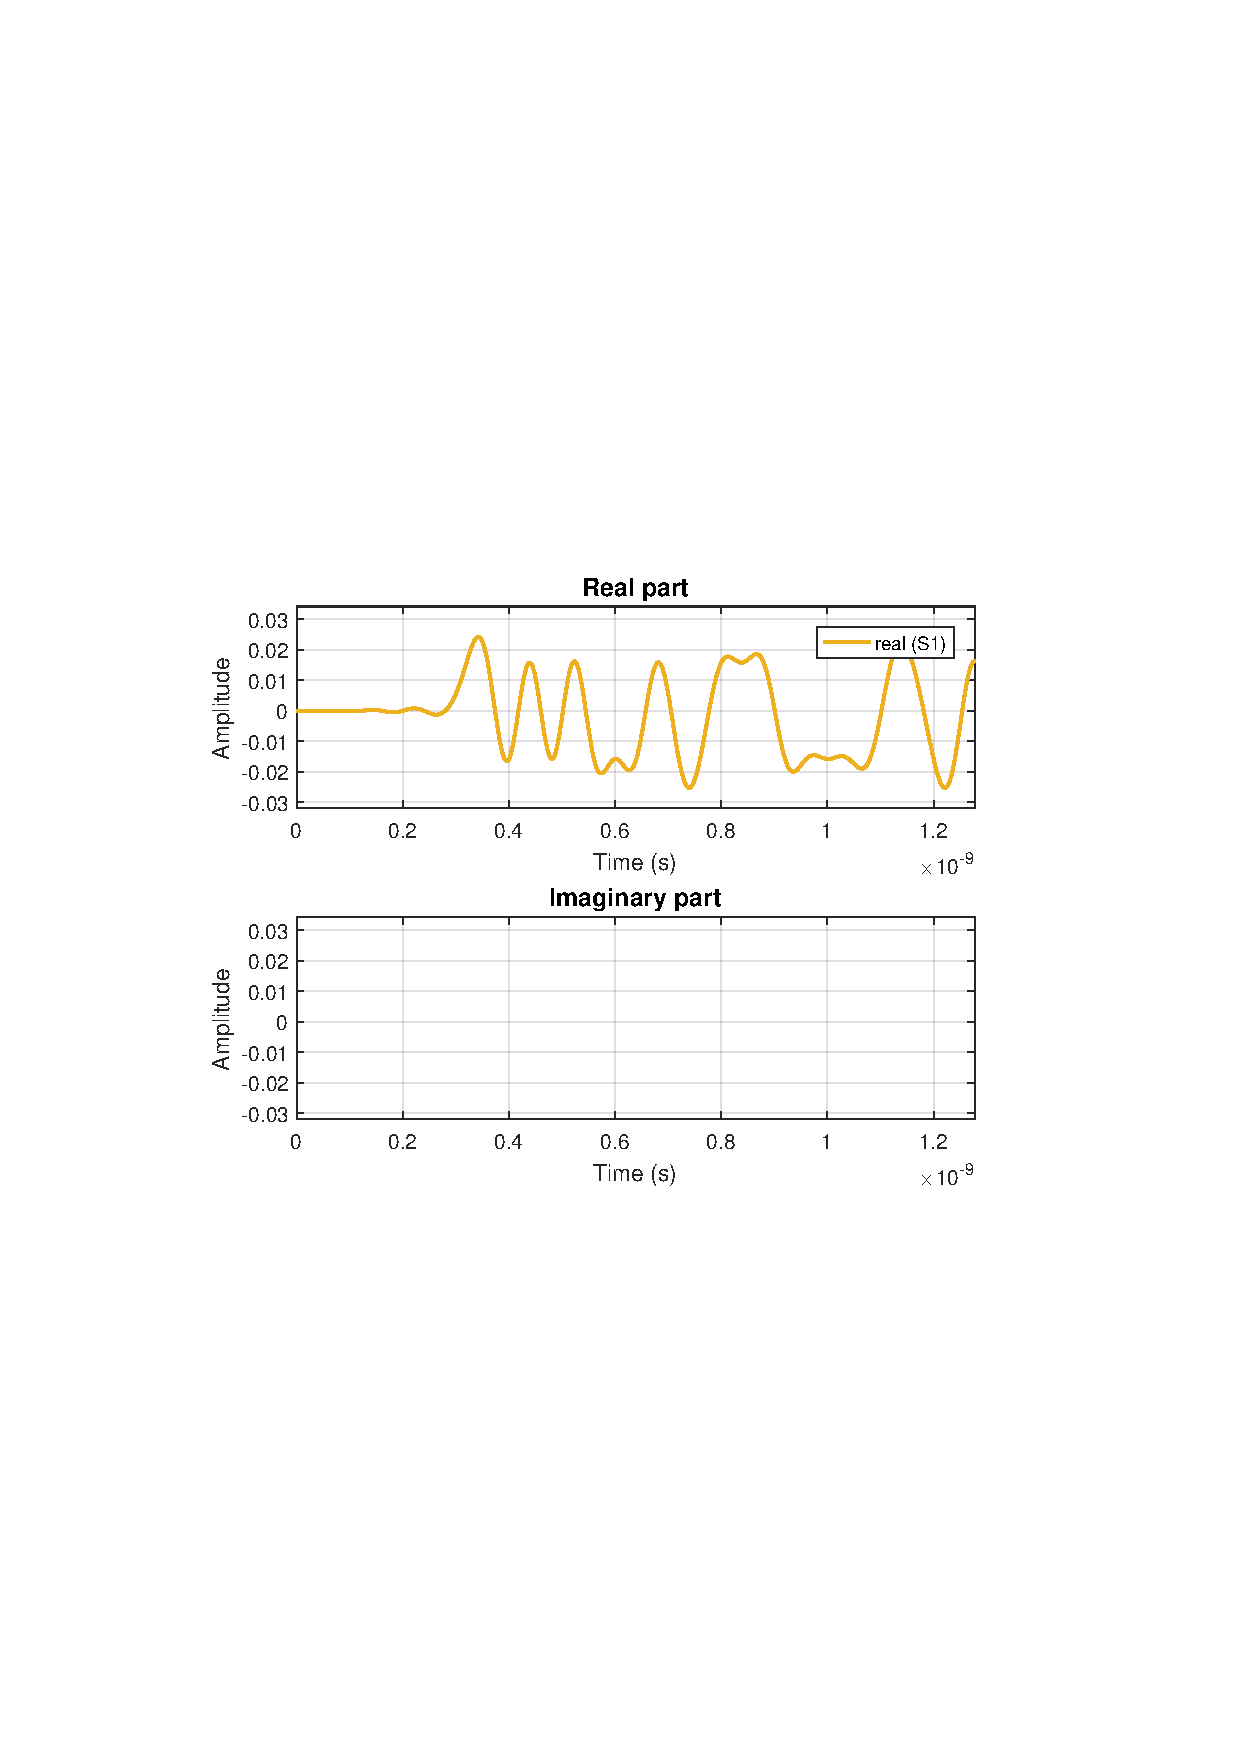
\includegraphics[width=\linewidth, trim= 0mm 100mm 0mm 100mm, clip]{sentsig.pdf}
%\caption{Sent signal.}
%\label{fig:bsin1}
%\end{figure}
%
%\begin{figure}[H]
%\centering
%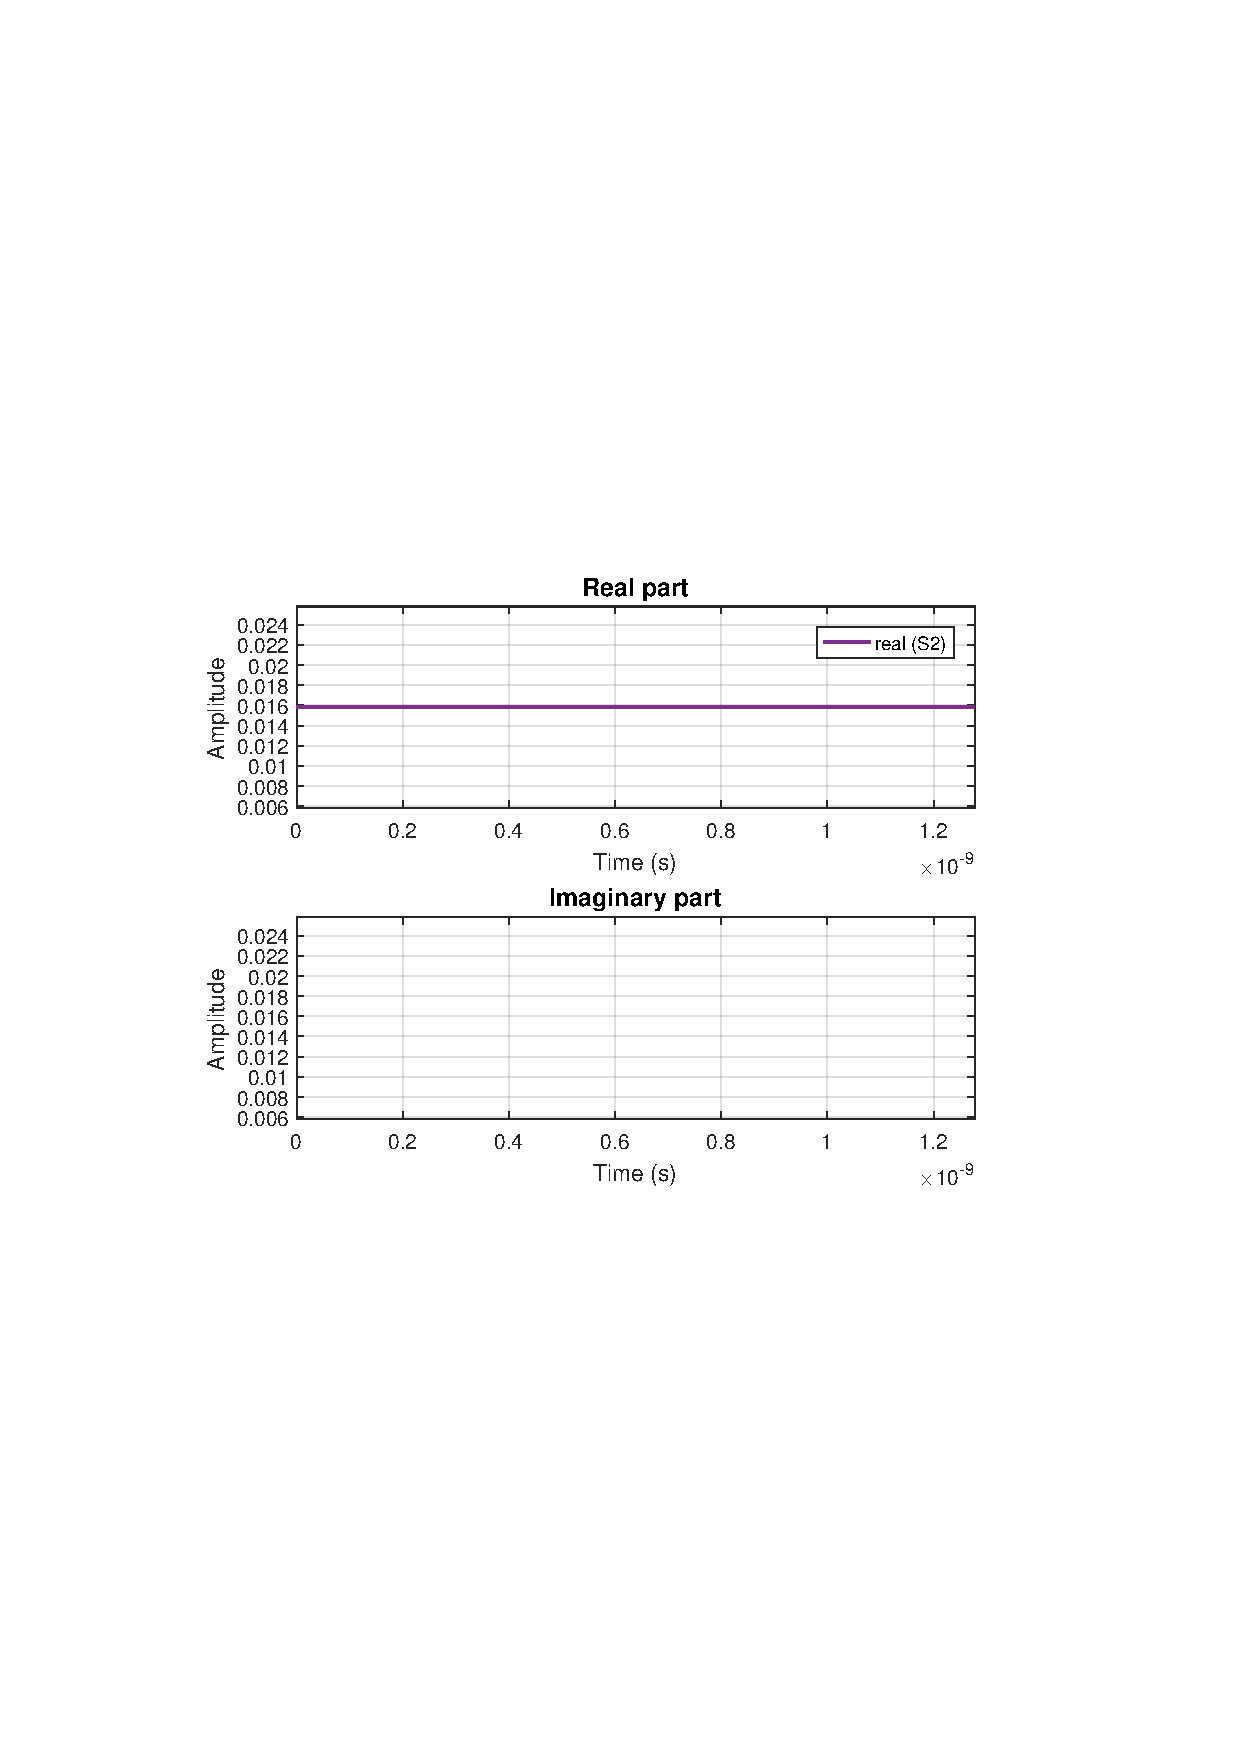
\includegraphics[width=\linewidth, trim= 0mm 100mm 0mm 100mm, clip]{lo.pdf}
%\caption{Sent local oscillator.}
%\label{fig:bsin2}
%\end{figure}
%
%\begin{figure}[H]
%\centering
%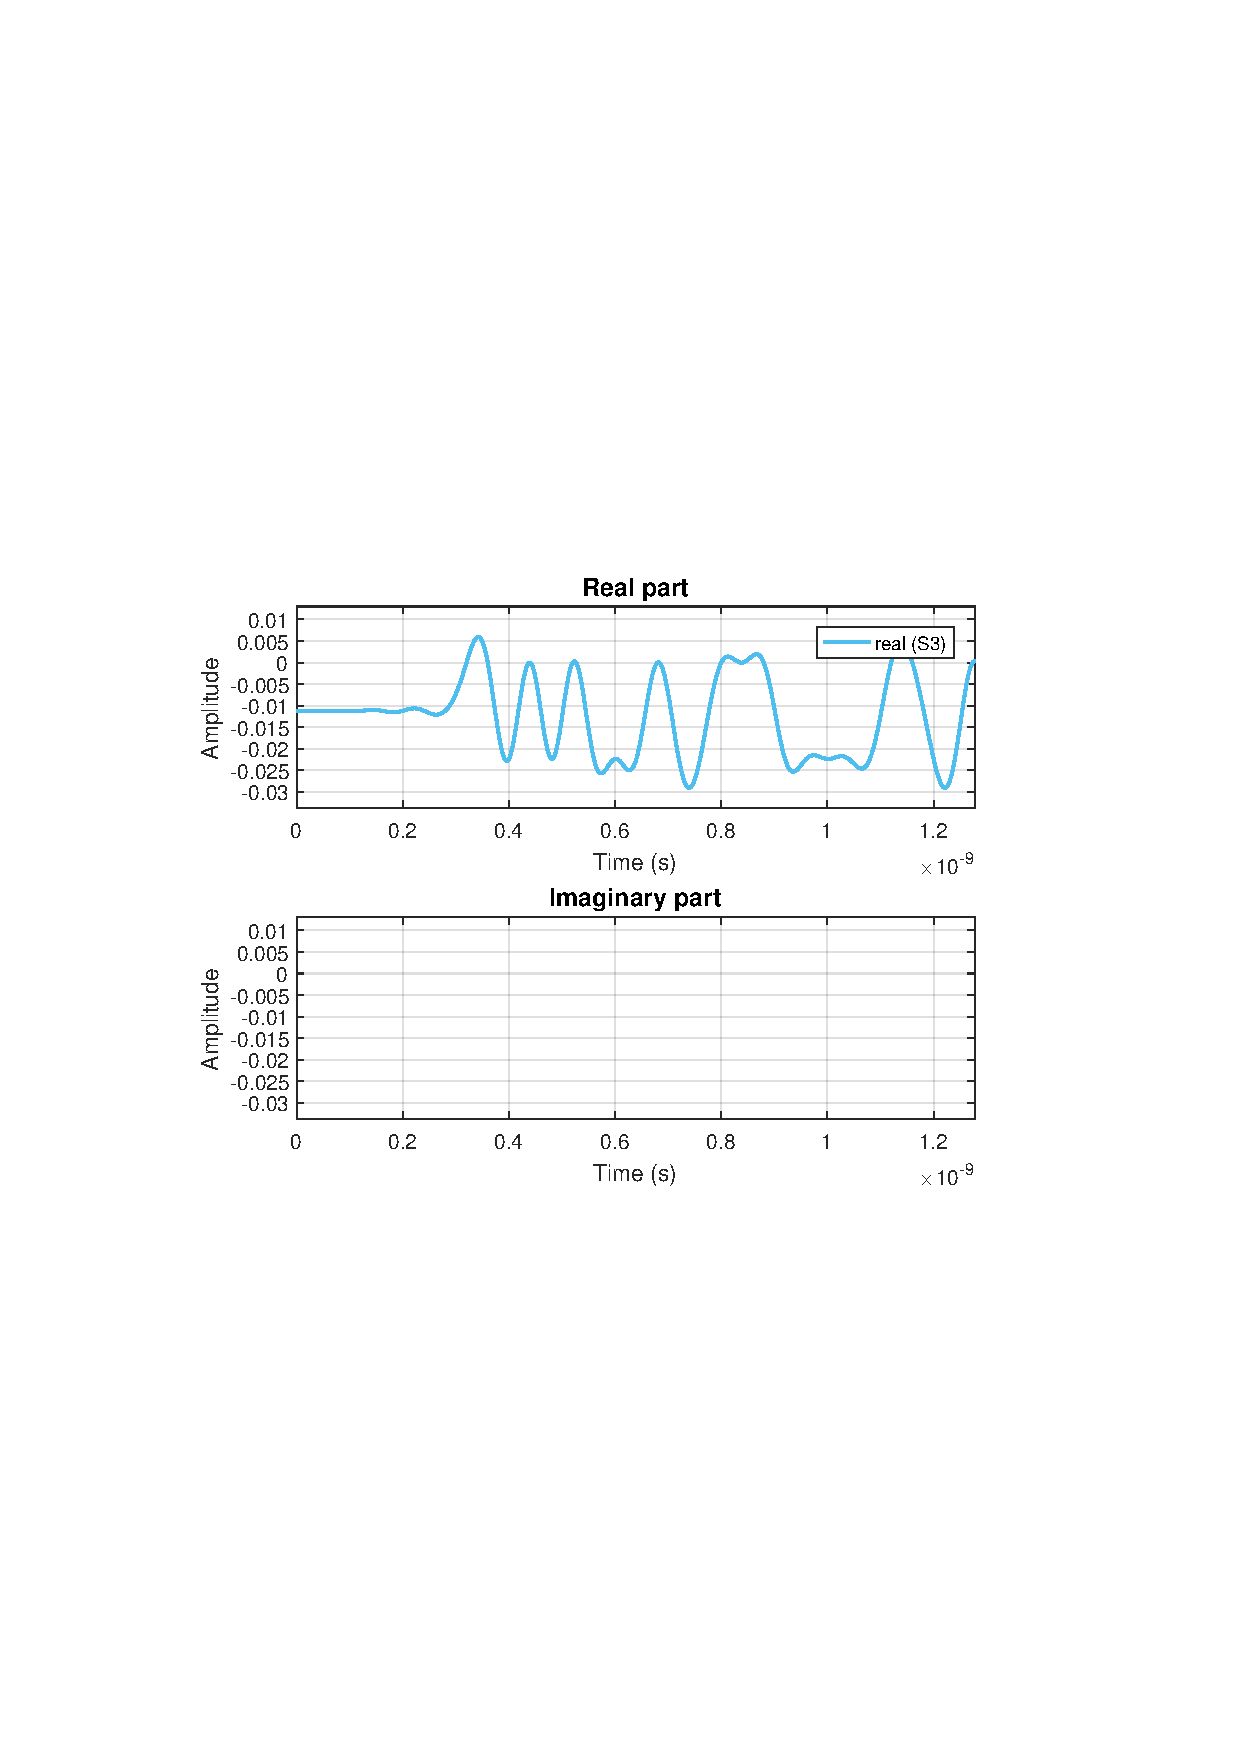
\includegraphics[width=\linewidth, trim= 0mm 100mm 0mm 100mm, clip]{bs1.pdf}
%\caption{First output of the beam-splitter.}
%\label{fig:bsout1}
%\end{figure}
%
%\begin{figure}[H]
%\centering
%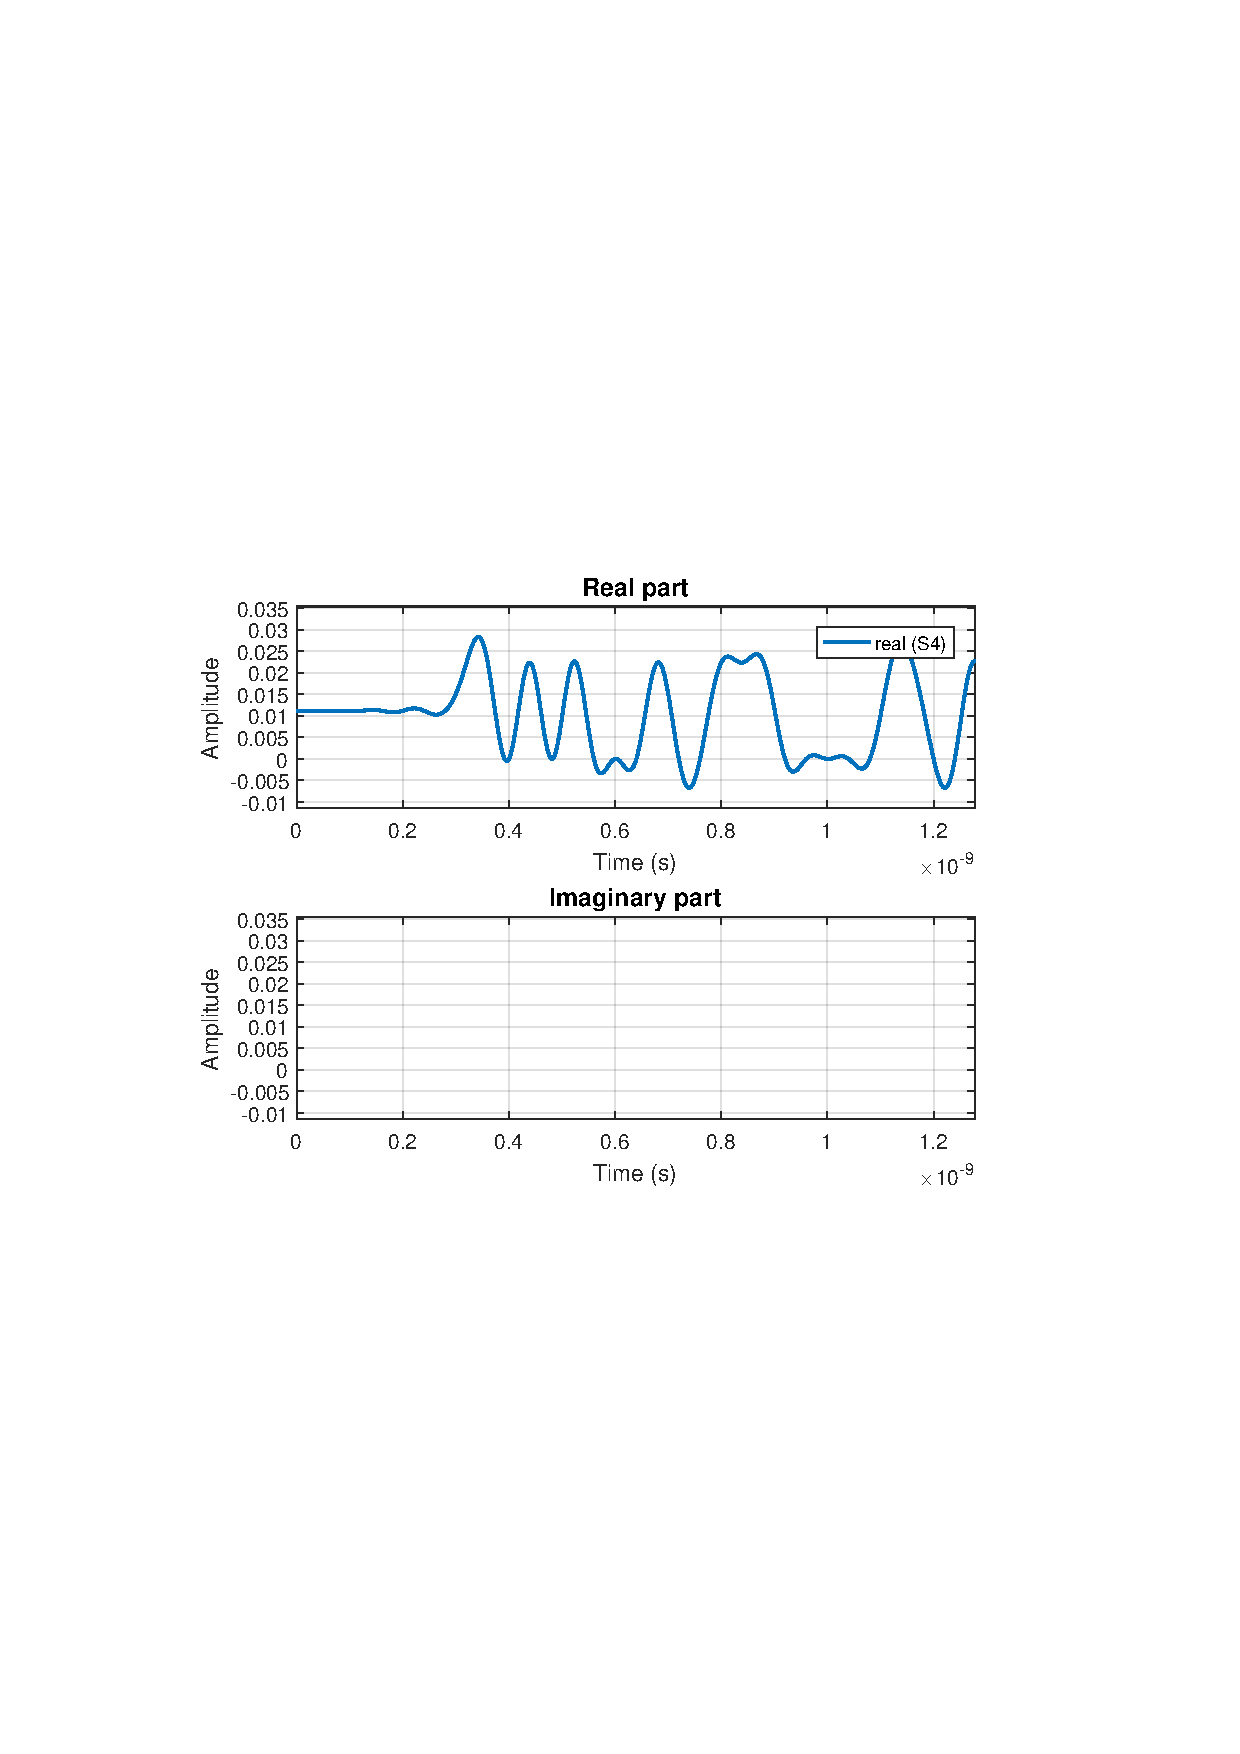
\includegraphics[width=\linewidth, trim= 0mm 100mm 0mm 100mm, clip]{bs2.pdf}
%\caption{Second output of the beam-splitter.}
%\label{fig:bsout2}
%\end{figure}

\subsection{Photodiode}

\subsubsection*{Input Parameters}

\begin{multicols}{2}
	\begin{itemize}
		\item setResponsivity
	\end{itemize}
\end{multicols}

\subsubsection*{Functional Description}

This block accepts two complex signals and outputs two real signals built from an evaluation of the power of the input signals.

\subsubsection*{Input Signals}

\textbf{Number}: 2

\textbf{Type}: Complex signal (ContinuousTimeContiousAmplitude)

\subsubsection*{Output Signals}

\textbf{Number}: 2

\textbf{Type}: Real signal (ContinuousTimeContiousAmplitude)

%This block takes one complex optical bandpass signal input and outputs one real electrical signal, taking into account the power of the input signal (correcting it in accordance with the Bandpass signal conversion) and the responsitivity of the photodiodes being simulated.
%\par
%The following code is run for every value in the input signal.
%
%\begin{verbatim}
%		t_complex x1;
%		inputSignals[0]->bufferGet(&x1);
%		t_real x1r = real(x1);
%		t_real x1i = imag(x1);
%		t_real radius = 0.0003;
%		t_real E0 = 8.854187817e-12;
%
%		t_real power = 2 * SPEED_OF_LIGHT * PI * radius*radius * E0 * (x1r*x1r + x1i*x1i) * 0.25;
%		t_real current = 1 * power;
%
%		outputSignals[0]->bufferPut(current);
%\end{verbatim}
%
%As shown in Figure~\ref{fig:simulatedsystem}, two photodiodes are used for the input of the Homodyne detector, taking for input the signals presented in Figures~\ref{fig:bsout1}~and~\ref{fig:bsout2}, these blocks output the signals presented in Figures~\ref{fig:photod1}~and~\ref{fig:photod2}.
%
%\begin{figure}[H]
%\centering
%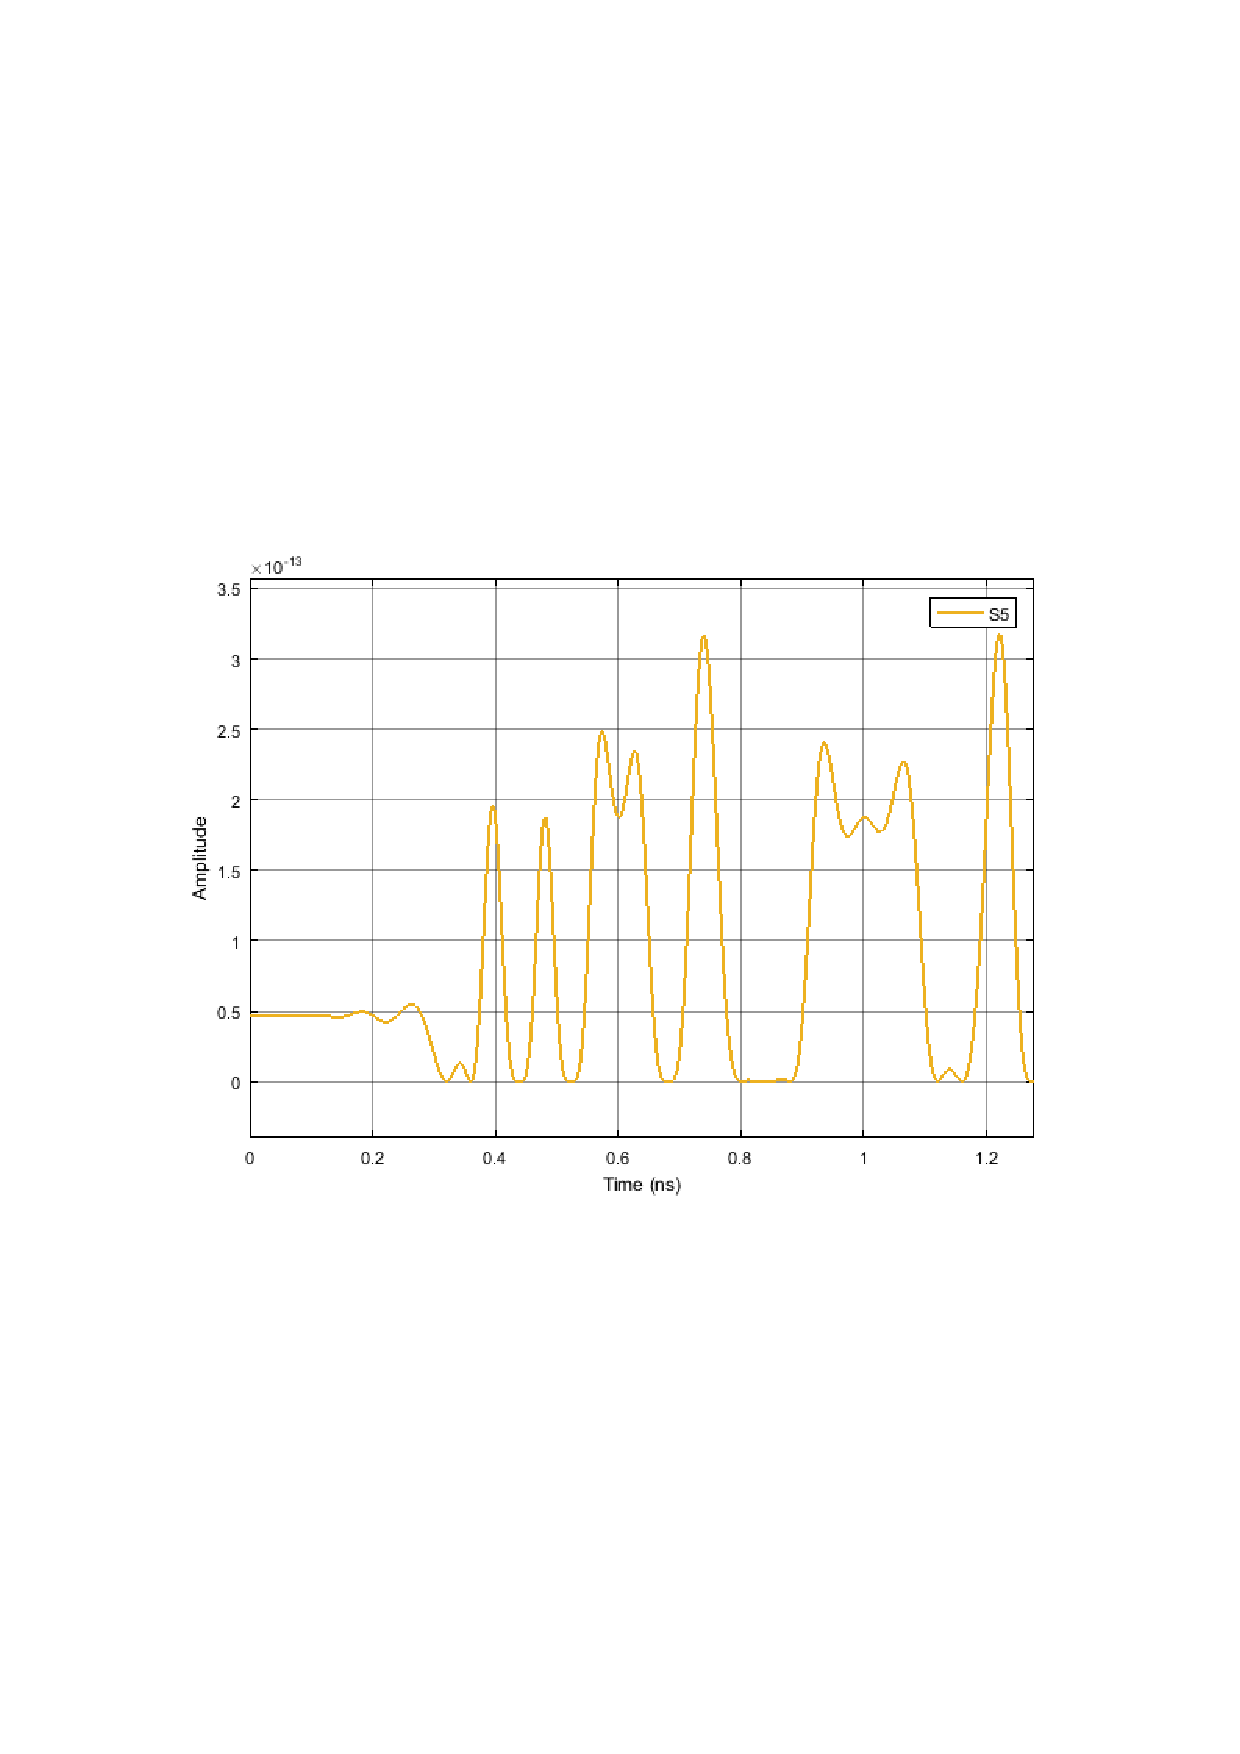
\includegraphics[width=\linewidth, trim= 0mm 100mm 0mm 100mm, clip]{photod1.pdf}
%\caption{Output of the first photo-diode.}
%\label{fig:photod1}
%\end{figure}
%
%\begin{figure}[H]
%\centering
%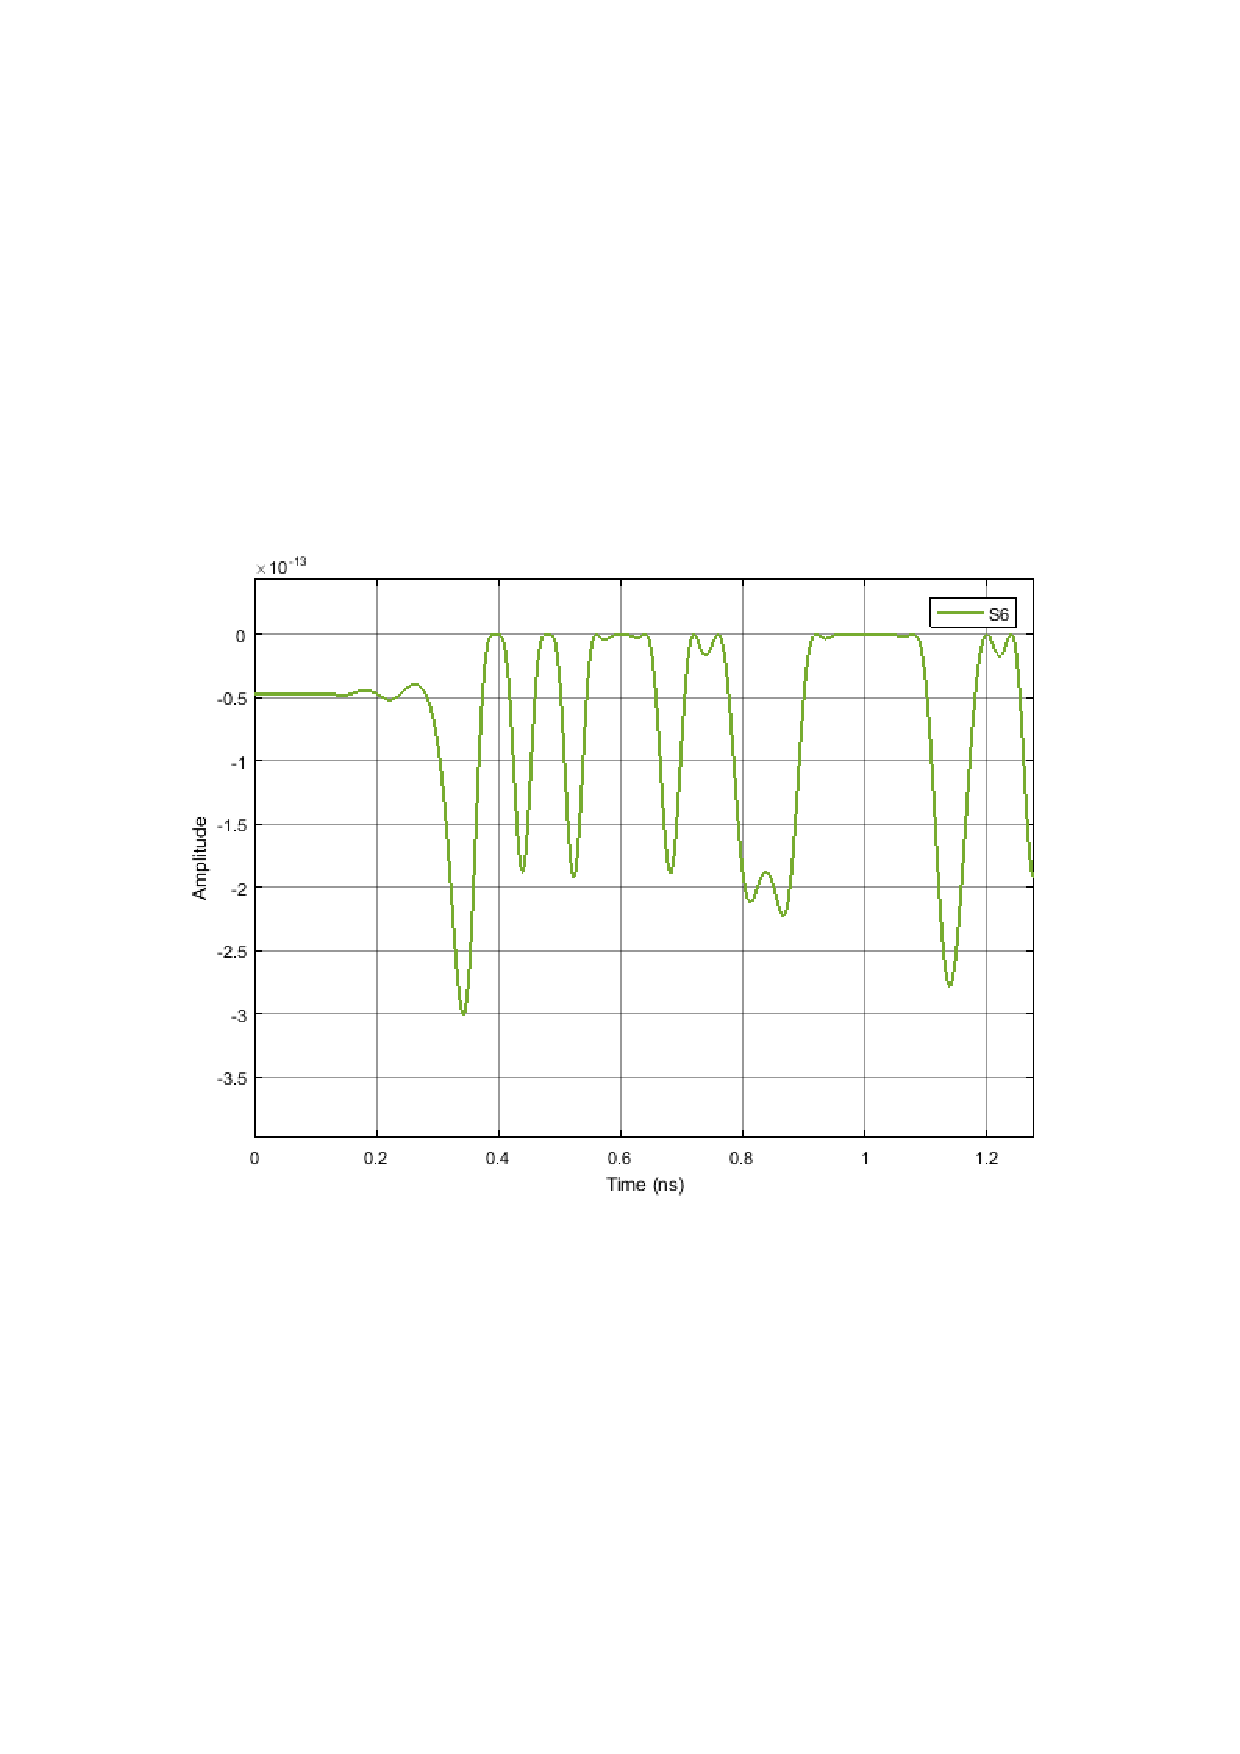
\includegraphics[width=\linewidth, trim= 0mm 100mm 0mm 100mm, clip]{photod2.pdf}
%\caption{Output of the second photo-diode.}
%\label{fig:photod2}
%\end{figure}


\subsection{Subtractor}

\subsubsection*{Input Parameters}

This block has no input parameters.

\subsubsection*{Functional Description}

This block accepts two real signals and outputs one real signals built from subtracting the value of the input signals.

\subsubsection*{Input Signals}

\textbf{Number}: 2

\textbf{Type}: Real signal (ContinuousTimeContiousAmplitude)

\subsubsection*{Output Signals}

\textbf{Number}: 1

\textbf{Type}: Real signal (ContinuousTimeContiousAmplitude)


%This block takes two real electrical signals, subtracts them and outputs one real electrical signal.
%\par
%The following code is run for every pair of values in the input signals.
%
%
%\begin{verbatim}
%		t_real x1;
%		inputSignals[0]->bufferGet(&x1);
%		t_real x2;
%		inputSignals[1]->bufferGet(&x2);
%
%		t_real out = x1 - x2;
%
%		outputSignals[0]->bufferPut(out);
%\end{verbatim}
%
%This block takes for input the signals presented in Figures~\ref{fig:photod1}~and~\ref{fig:photod2}, and outputs the signal presented in Figure~\ref{fig:subract}.
%
%\begin{figure}[H]
%\centering
%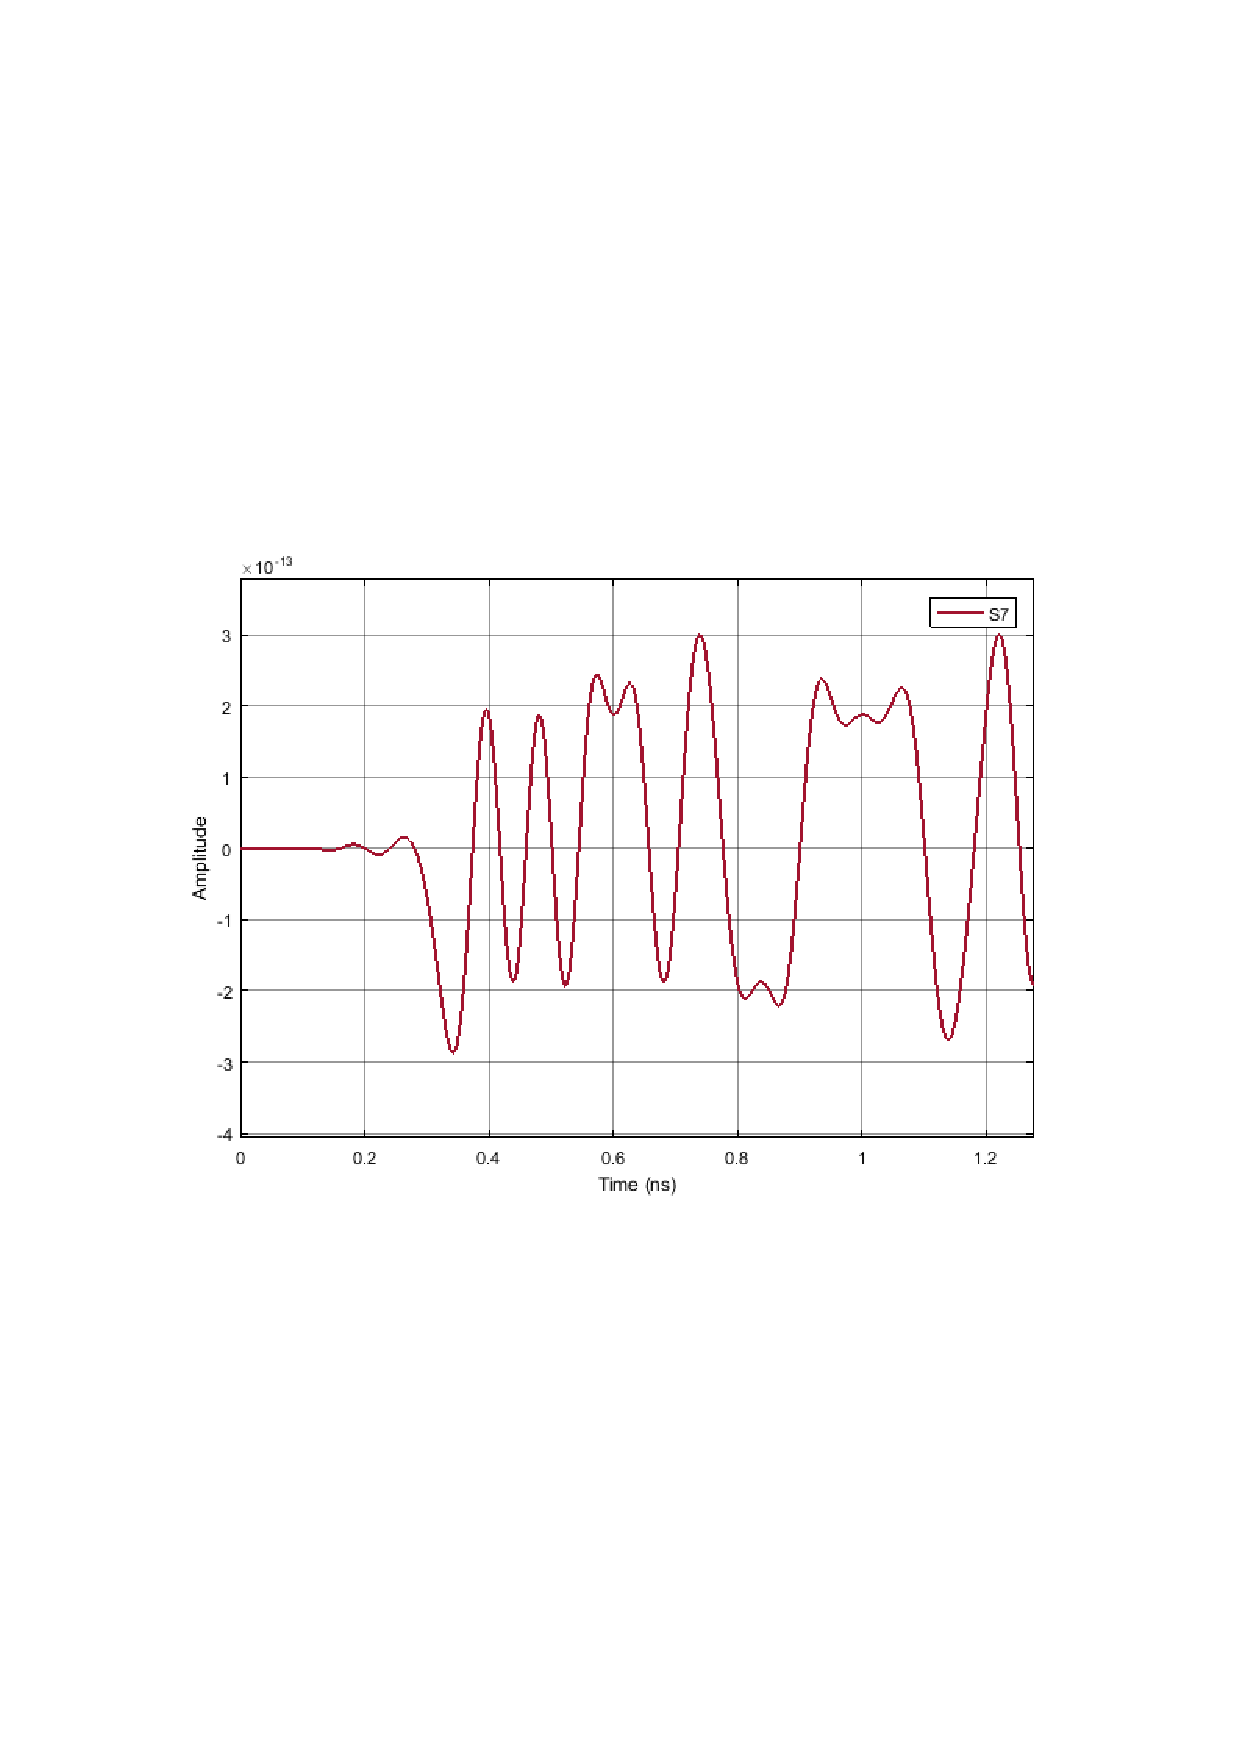
\includegraphics[width=\linewidth, trim= 0mm 100mm 0mm 100mm, clip]{subtracted.pdf}
%\caption{Subtraction of the two photo-currents.}
%\label{fig:subract}
%\end{figure}

\subsection{Amplifier}

\subsubsection*{Input Parameters}

\begin{multicols}{2}
	\begin{itemize}
		\item setAmplification
		\item setNoiseAmplitude
	\end{itemize}
\end{multicols}

\subsubsection*{Functional Description}

This block accepts one real signal and outputs one real signal built from multiplying the input signals by a predetermined value. This block also adds random gaussian distributed noise with a user defined amplitude. The multiplying factor and noise amplitude are defined by the values of \textit{Amplification} and \textit{NoiseAmplitude} respectively.

\subsubsection*{Input Signals}

\textbf{Number}: 1

\textbf{Type}: Real signal (ContinuousTimeContiousAmplitude)

\subsubsection*{Output Signals}

\textbf{Number}: 1

\textbf{Type}: Real signal (ContinuousTimeContiousAmplitude)


%This block takes one real electrical input and, amplifies it's amplitude and outputs one real electrical signal.
%\par
%The following code is run for every value in the input signal.
%
%\begin{verbatim}
%		t_real signalValue;
%		inputSignals[0]->bufferGet(&signalValue);
%		t_real out = signalValue*10000;
%
%		outputSignals[0]->bufferPut(out);
%\end{verbatim}
%
%This block takes for input the signal presented in Figure~\ref{fig:subract}, and outputs the signal presented in Figure~\ref{fig:amplf}.
%
%\begin{figure}[H]
%\centering
%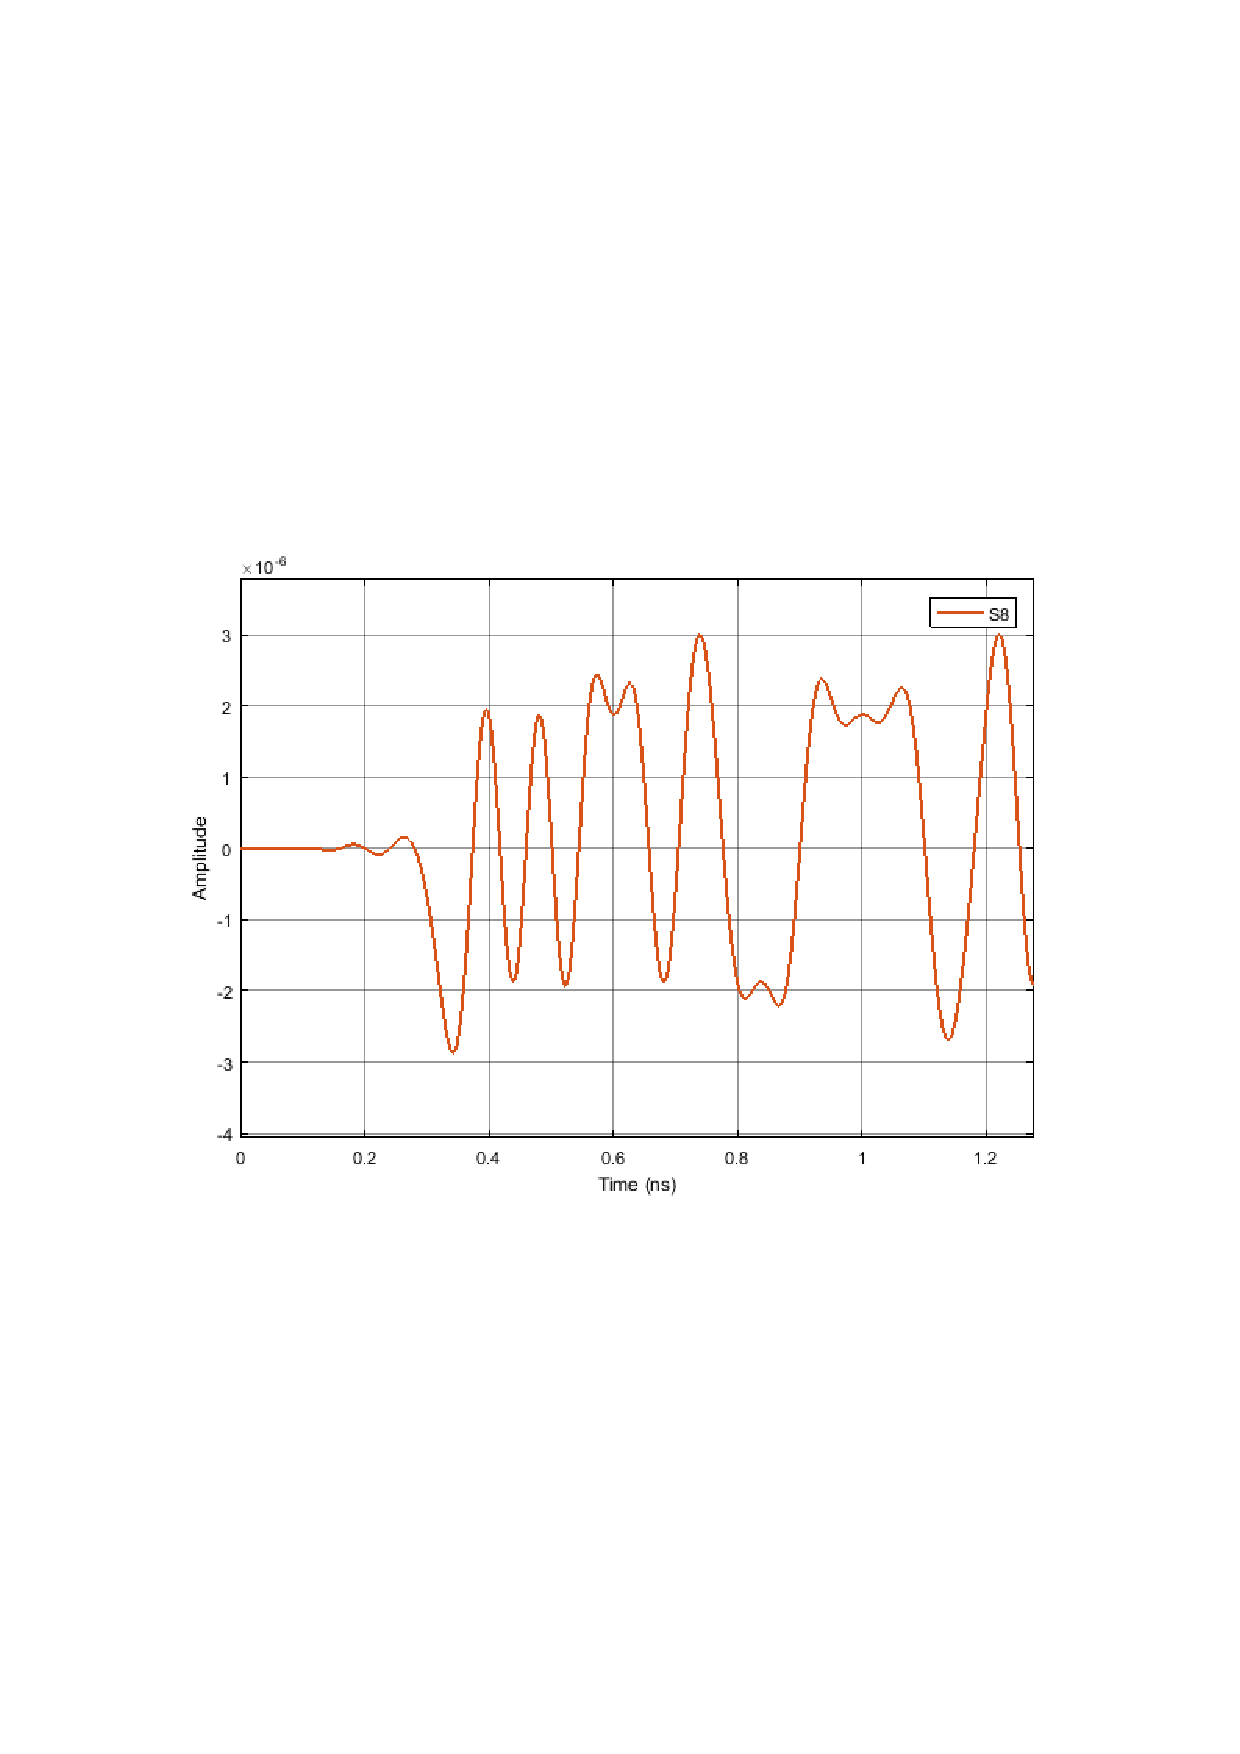
\includegraphics[width=\linewidth, trim= 0mm 100mm 0mm 100mm, clip]{amplified.pdf}
%\caption{Amplification of the photo-current.}
%\label{fig:amplf}
%\end{figure}

\subsection{Discretizer}

\subsubsection*{Input Parameters}

\begin{multicols}{2}
	\begin{itemize}
		\item setSamplingRate
	\end{itemize}
\end{multicols}

\subsubsection*{Functional Description}

This block accepts one real continuous signal and outputs one real discrete signal built from a sampling of the input signals with a predetermined sampling rate. The sampling rate is defined by the value \textit{SamplingRate}.

\subsubsection*{Input Signals}

\textbf{Number}: 1

\textbf{Type}: Real signal (ContinuousTimeContiousAmplitude)

\subsubsection*{Output Signals}

\textbf{Number}: 1

\textbf{Type}: Real signal (DiscreteTimeContiousAmplitude)


%This block takes one real, continuous electrical input and samples it at a rate of one sample per bit period, outputting a real discrete signal.
%\par
%The following code is run for every value in the input signal.
%
%\begin{verbatim}
%		t_real signalValue;
%		inputSignals[0]->bufferGet(&signalValue);
%		auxint = auxint + 1;
%
%		if (auxint == period)
%		{
%			auxint = 0;
%			out = signalValue;
%			outputSignals[0]->bufferPut(out);
%		}
%\end{verbatim}
% 
%Note that the discretization is accomplished by the if clause, that causes that only one value per bit period will be saved.
%\par
%This block takes for input the signal presented in Figure~\ref{fig:amplf}, and outputs the signal presented in Figure~\ref{fig:discrt}.
%
%\begin{figure}[H]
%\centering
%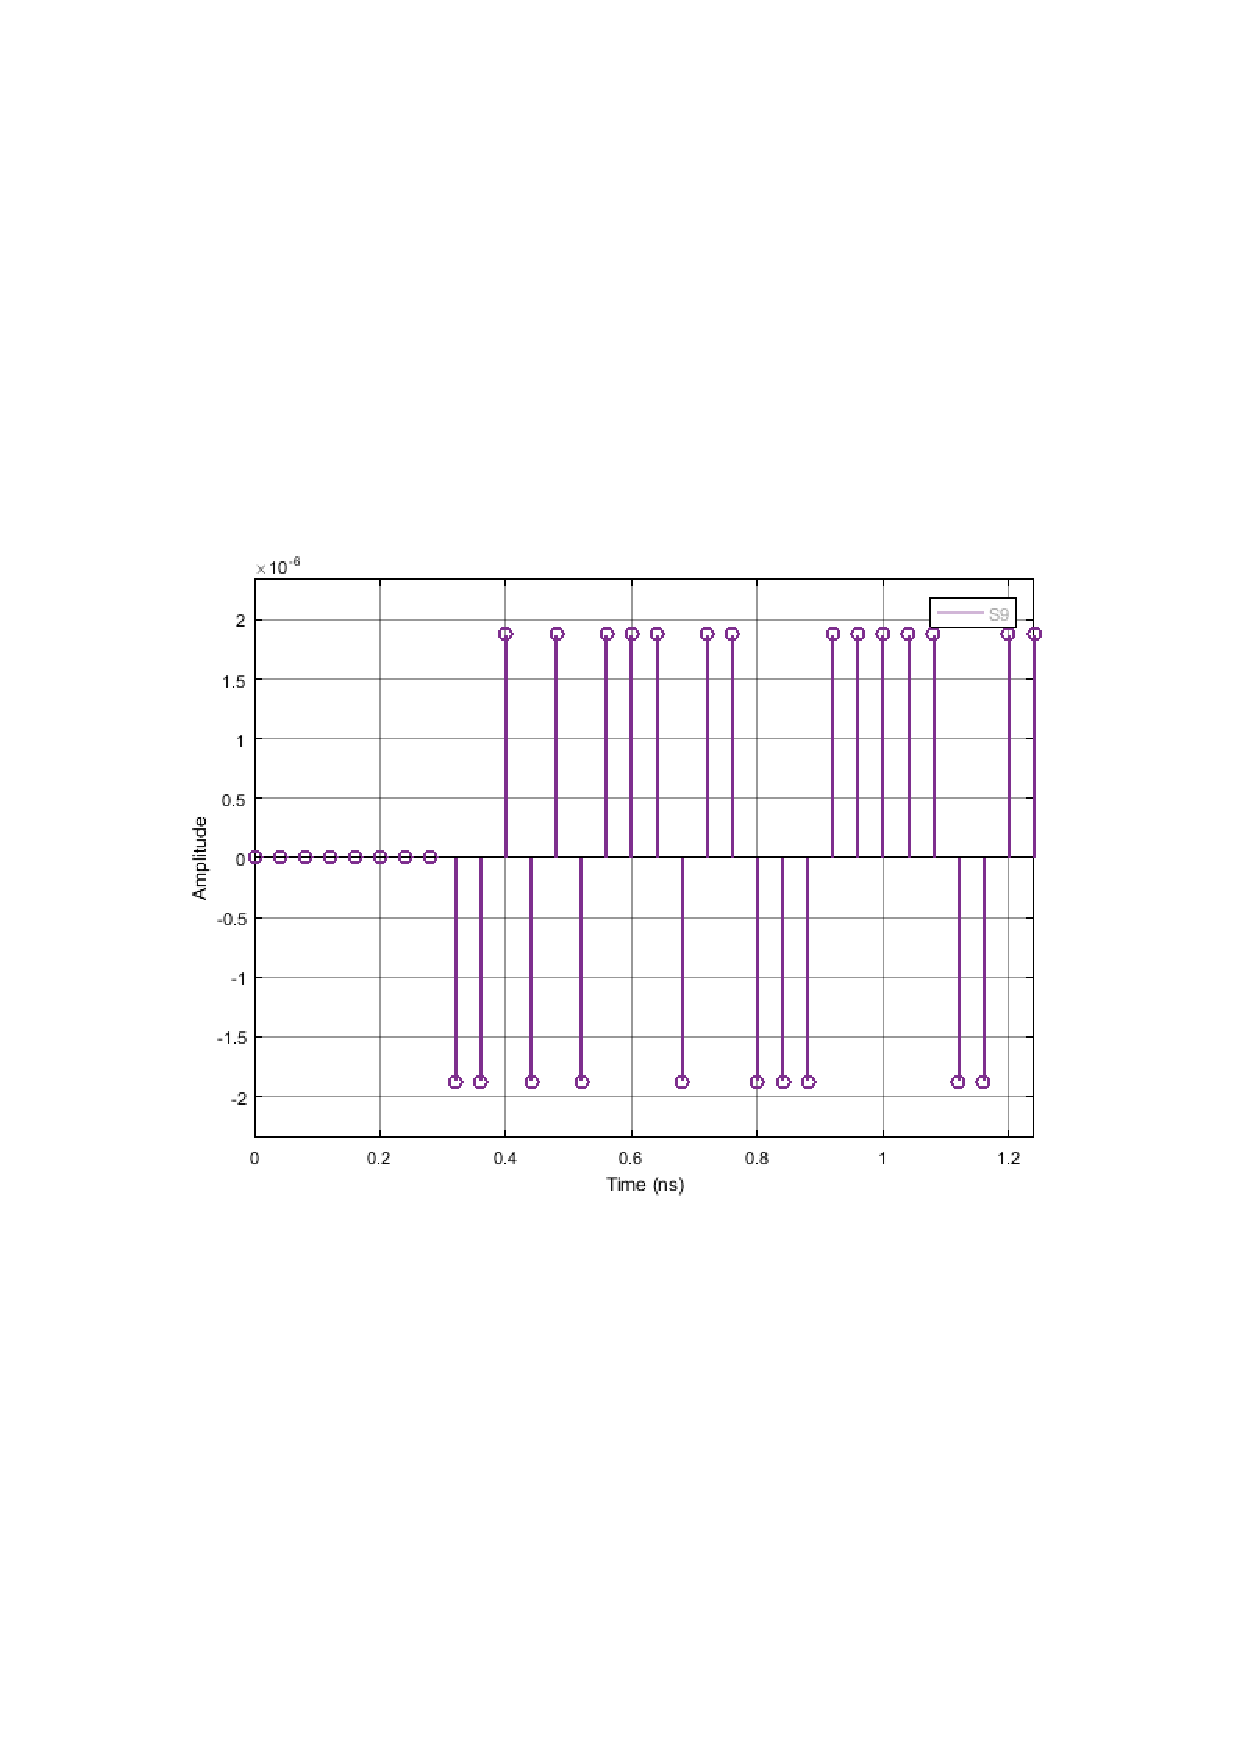
\includegraphics[width=\linewidth, trim= 0mm 100mm 0mm 100mm, clip]{discretized.pdf}
%\caption{Discretization of the amplified signal.}
%\label{fig:discrt}
%\end{figure}


\subsection{Delayer}

\subsubsection*{Input Parameters}

\begin{multicols}{2}
	\begin{itemize}
		\item setDelay
	\end{itemize}
\end{multicols}

\subsubsection*{Functional Description}

This block accepts one real discrete signal and outputs one real discrete signal discarding a predetermined number of samples of the beginning of the input signal. The number of samples discarded rate is defined by the value \textit{Delay}.

\subsubsection*{Input Signals}

\textbf{Number}: 1

\textbf{Type}: Real signal (DiscreteTimeContiousAmplitude)

\subsubsection*{Output Signals}

\textbf{Number}: 1

\textbf{Type}: Real signal (DiscreteTimeContiousAmplitude)


%This block takes in one real discrete input and discards the first few values, such that the output signal is composed only by values related to the bit value being sent and not due to the convolution of sine waves.
%\par
%The following code is run for every value in the input signal.
%\begin{verbatim}
%		t_real signalValue;
%		inputSignals[0]->bufferGet(&signalValue);
%		auxint = auxint + 1;
%
%		if (auxint >= delay)
%		{
%			out = signalValue;
%			outputSignals[0]->bufferPut(out);
%		}
%\end{verbatim}
%
%This block takes for input the signal presented in Figure~\ref{fig:discrt}, and outputs the signal presented in Figure~\ref{fig:delay}.
%
%\begin{figure}[H]
%\centering
%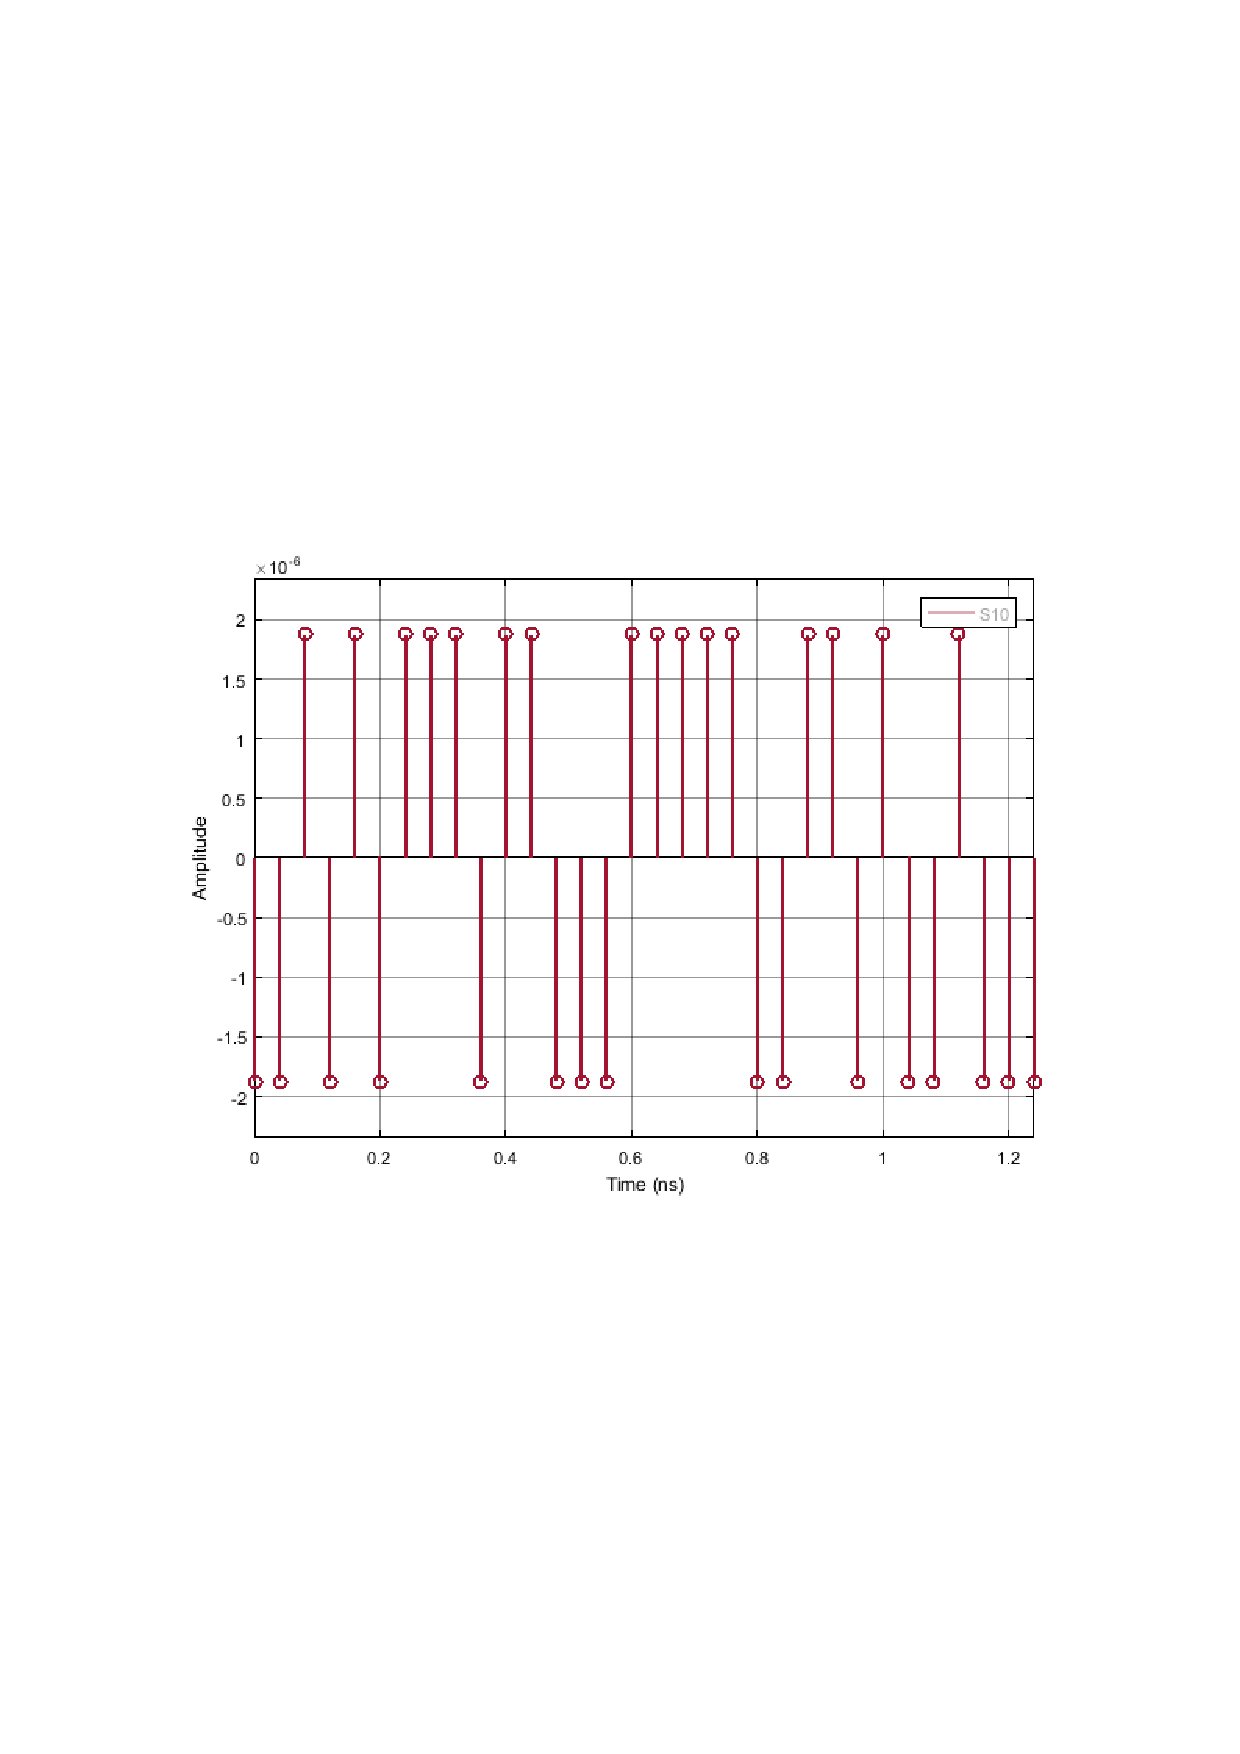
\includegraphics[width=\linewidth, trim= 0mm 100mm 0mm 100mm, clip]{delayed.pdf}
%\caption{Removal of the first samples.}
%\label{fig:delay}
%\end{figure}

\subsection{Bit decider}

\subsubsection*{Input Parameters}

\begin{multicols}{2}
	\begin{itemize}
		\item setPosReferenceValue
		\item setNegReferenceValue
	\end{itemize}
\end{multicols}

\subsubsection*{Functional Description}

This block accepts one real discrete signal and outputs a binary string, outputting a 1 if the input sample is above the predetermined reference level and 0 if it is below another reference value The reference values are defined by the values of \textit{PosReferenceValue} and \textit{NegReferenceValue}.

\subsubsection*{Input Signals}

\textbf{Number}: 1

\textbf{Type}: Real signal (DiscreteTimeContiousAmplitude)

\subsubsection*{Output Signals}

\textbf{Number}: 1

\textbf{Type}: Binary (DiscreteTimeDiscreteAmplitude)


%This block takes in one real discrete input and outputs a binary string, attributing values in accordance to the relation between the input values and a internal reference value.
%\par
%The following code is run for every value in the input signal.
%\begin{verbatim}
%		t_real signalValue;
%		inputSignals[0]->bufferGet(&signalValue);
%		if (signalValue>0)
%		{
%			outputSignals[0]->bufferPut(1);
%		}
%		else
%		{
%			outputSignals[0]->bufferPut(0);
%		}
%\end{verbatim}
%
%Note that in this case the reference value is merely 0, in the future this value will need to take into account the noise level.
%\par
%This block takes for input the signal presented in Figure~\ref{fig:delay}, and outputs the signal presented in Figure~\ref{fig:decision}.
%
%\begin{figure}[H]
%\centering
%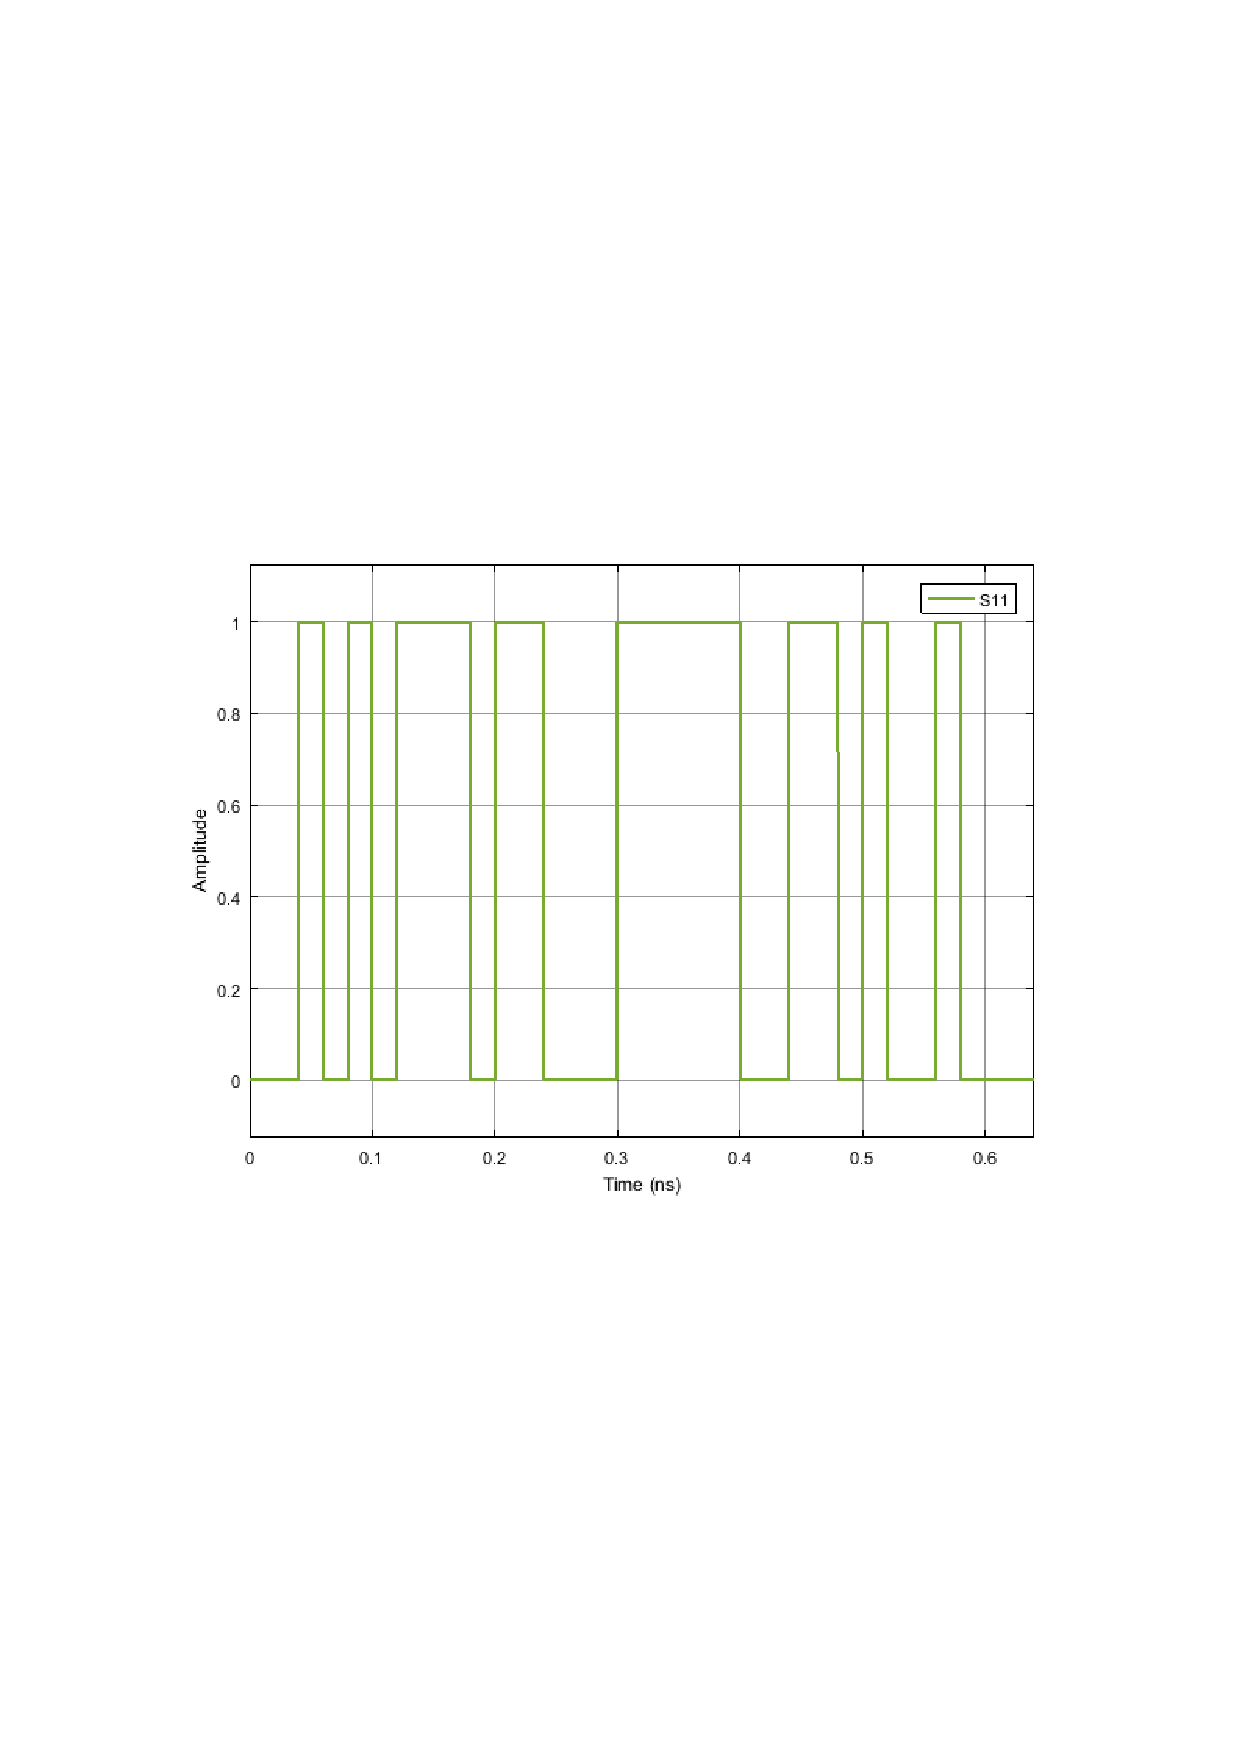
\includegraphics[width=\linewidth, trim= 0mm 100mm 0mm 100mm, clip]{recvkey.pdf}
%\caption{Result of the bit decision, reconstructed key.}
%\label{fig:decision}
%\end{figure}

\subsection{Bit Error-Rate}

\subsubsection*{Input Parameters}

\begin{multicols}{2}
	\begin{itemize}
		\item setZ
	\end{itemize}
\end{multicols}

\subsubsection*{Functional Description}

This block accepts two binary strings and outputs a binary string, outputting a 1 if the two input samples are equal to each other and 0 if not. This block also outputs a \textit{.txt} file with a report of the calculate BER as well as the estimated Confidence bounds for a given probability $1-\alpha$. The probability for the confidence bounds is determined by the $z_{1-\frac{\alpha}{2}}$ percentile of a standard gaussian distribution, value which has to be fed into the block.

\subsubsection*{Input Signals}

\textbf{Number}: 1

\textbf{Type}: Binary (DiscreteTimeDiscreteAmplitude)

\subsubsection*{Output Signals}

\textbf{Number}: 1

\textbf{Type}: Binary (DiscreteTimeDiscreteAmplitude)


%This block takes as inputs two binary strings and evaluates the number of coincidences, outputting a copy of of the inputs (this output is of no importance) and a .txt file with a report of the obtained results.
%\par
%The following code is responsible for the functioning of the block:
%\begin{verbatim}
%int ready = inputSignals[0]->ready();
%
%	int space = outputSignals[0]->space();
%
%	int process = min(ready, space);
%
%	float NumberOfBits = recievedbits;
%	float Coincidences = coincidences;
%
%	float BER;
%	BER = (NumberOfBits - Coincidences) / NumberOfBits * 100;
%
%	if (process == 0)
%	{
%		ofstream myfile;
%		myfile.open("BER.txt");
%		myfile << "BER=" << BER<<"\%";
%		myfile.close();
%		return false;
%	}
%
%
%
%	for (int i = 0; i < process; i++) {
%
%		t_binary signalValue;
%		inputSignals[0]->bufferGet(&signalValue);
%		t_binary SignalValue;
%		inputSignals[1]->bufferGet(&SignalValue);
%
%		recievedbits++;
%
%		if (signalValue==SignalValue)
%		{
%			coincidences++;
%		}
%
%
%
%		outputSignals[0]->bufferPut(&signalValue);
%
%	}
%	return true;
%\end{verbatim}
%Note that the .txt file is only written when one the input signals is spent.
%\par
%This block takes for input the signals presented in Figures~\ref{fig:decision}~and~\ref{fig:sent}, and outputs the .txt file presented in Figure~\ref{fig:ber}.
%
%\begin{figure}[H]
%\centering
%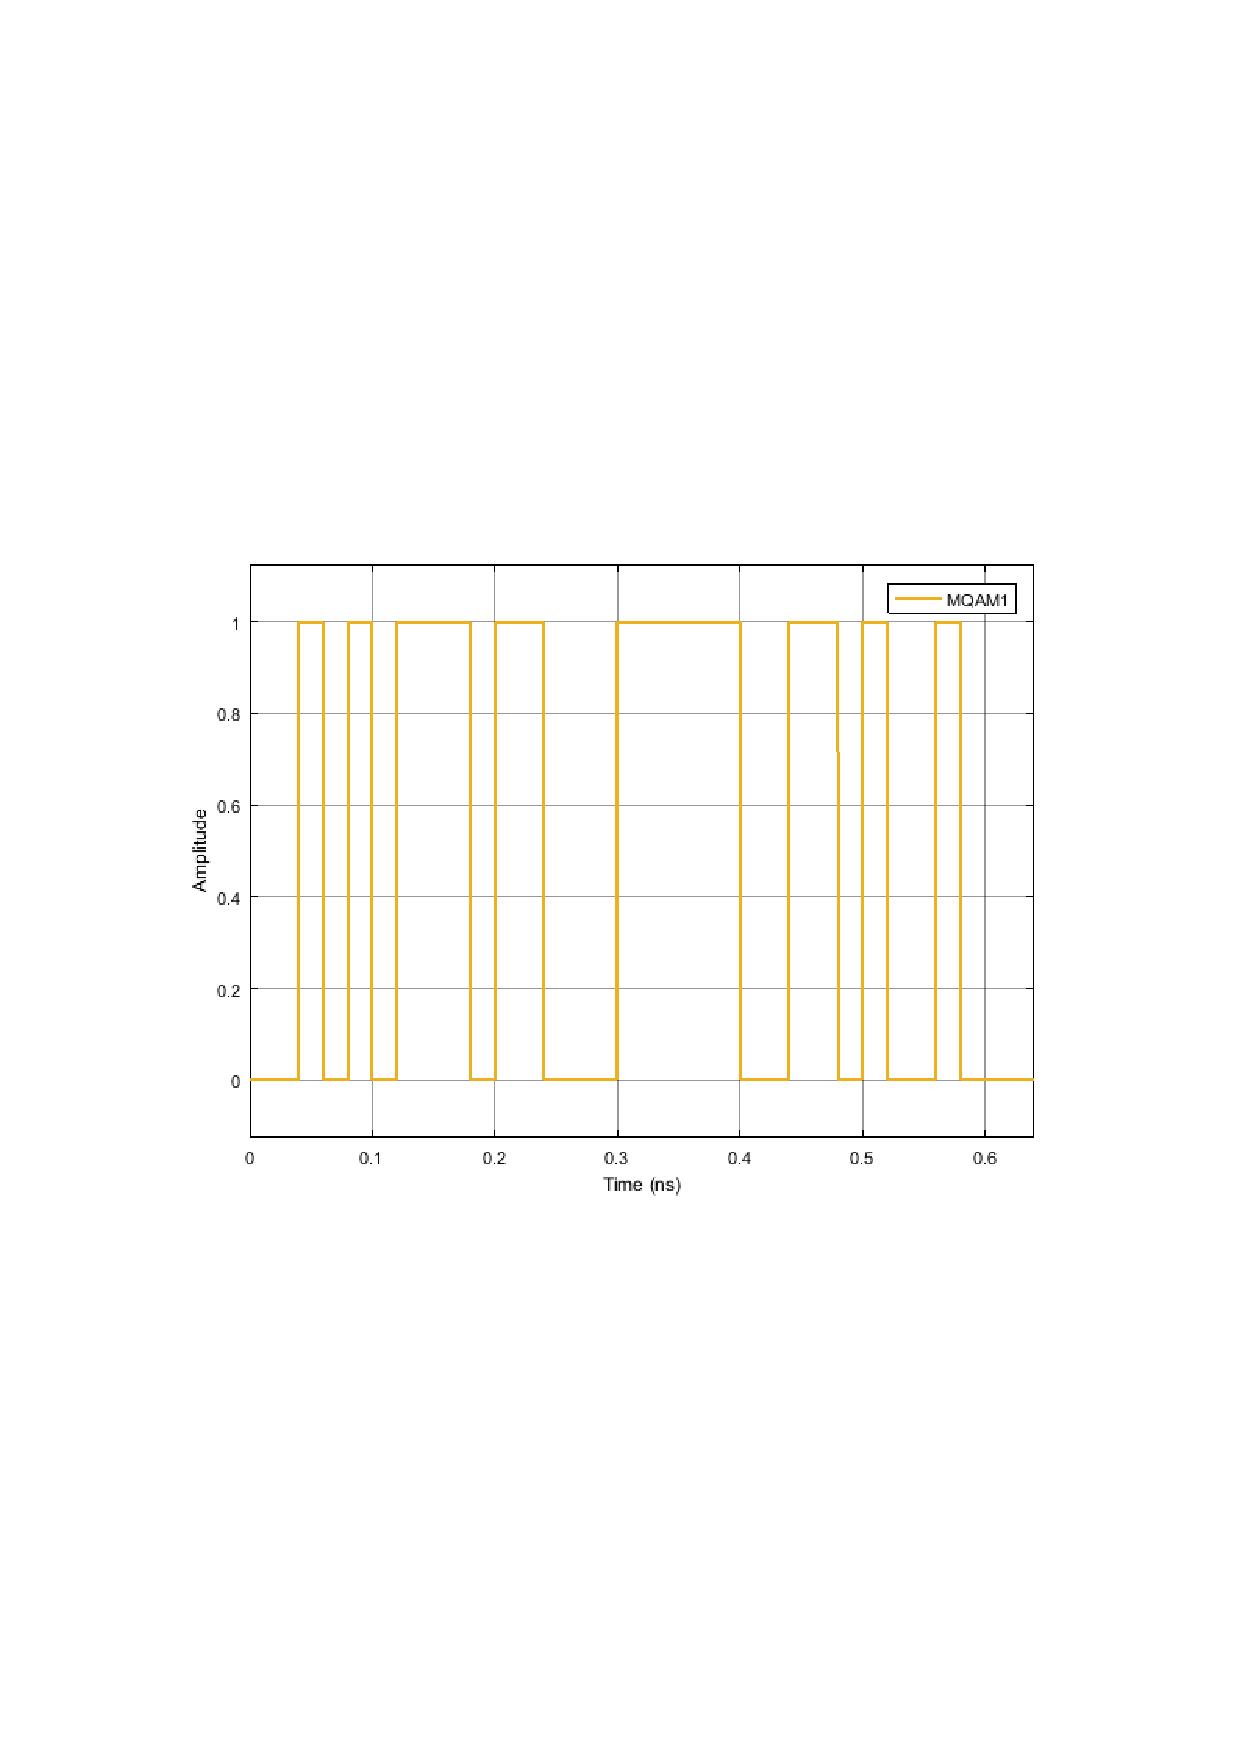
\includegraphics[width=\linewidth, trim= 0mm 100mm 0mm 100mm, clip]{sentkey.pdf}
%\caption{Sent bit sequence.}
%\label{fig:sent}
%\end{figure}
%
%\begin{figure}[H]
%\centering
%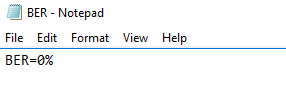
\includegraphics{ber.png}
%\caption{Image of the report generated by the BER block.}
%\label{fig:ber}
%\end{figure}



%\bibliographystyle{unsrt}
%\bibliography{bibliography}

\end{document}